\Chapter{Szürkeárnyalatos képek kiszínezése}

A szürkeárnyalatos kép és a megkapott címke térkép segítségével már az előző fejezetben ki tudtuk színezni a szegmenseket, viszont a kiszínezés az eredeti kép árnyalatait nem vette figyelembe. A fejezet célja hogy a színezést úgy valósítsuk meg, hogy az eredeti kép árnyalatait is megjelenítjük. A minél jobb eredmény elérésének érdekében az RGB és HSV színterekben is megvizsgáltam a problémát, ezeknek a vizsgálatoknak az eredménye a következő alfejezetekben található.

Maguk a színterek a színek matematikai ábrázolásai, lehetővé teszik a színek reprodukálható geometriai ábrázolását a 2D-3D terekben. A színterek a színmodellek és a leképezési függvények kombinációja, és információt tartalmaznak a kép egyes pixeleinek a színéről. A színes képek szegmentálására használt gyakori színterek az RGB, YIQ, HSV, CIE XYZ. \cite{colorspaces}

\Section{RGB}

Az RGB színterű képekben a kép minden egyes pixelét 3 színnel határozzuk meg:
\begin{itemize}
\item vörös (Red)
\item zöld (Green)
\item kék (Blue)
\end{itemize}
A paraméterek a szín intenzitását határozzák meg, az értékük egy 0-255 közötti egész szám. Ha mindegyik paraméterből a maximális, 255 értéket vesszük akkor a fehér színt, ha mindegyikből a minimális, az az a 0 értéket vesszük, akkor pedig a fekete színt kapjuk meg.  Egyszerűsége miatt a színtér széles körben elterjedt. \cite{colorspaces}

Szürkeárnyalatos képek esetén a 3 paraméter értéke megegyezik, így legtöbb esetben csak 1 értékkel szokták a kép pixeleit jelölni, tehát például szürkeárnyalatos képnél egy fekete színű pixel értéke 0.

Ahhoz, hogy egy szürkeárnyalatos képen színt tudjunk megjeleníteni, először át kell alakítanunk RGB színterűvé. Az átalakítást, hasonlóan az előző fejezetben bemutatott \texttt{color\_image} függvényhez, a \texttt{cv2} csomag \texttt{cvtColor} metódusával fogjuk megtenni.
\begin{python}
colored_image = cv2.cvtColor(resized_image, cv2.COLOR_GRAY2RGB)
\end{python}

Egy adott pixelre a színt a következő képlettel határozom meg:
\begin{align*}
 \text{new\_pixel\_color} & = (R, G, B) \\
 Y & = \text{grayscale\_image}[i][j]\\
 R_{ij} & = Y \cdot R / 255 \\
 G_{ij} & = Y \cdot G / 255 \\
 B_{ij} & = Y \cdot B / 255 \\
 \text{colored\_image}_{ij} & = (R_{ij}, G_{ij}, B_{ij})
\end{align*}
\noindent ahol az $i,j$ a kép adott pixelének az indexe.

A pixeleket a \texttt{numpy} csomag \texttt{multiply} függvényével színezem ki a következő kódrészletben látható módon.

\begin{python}
r, g, b = cv2.split(colored_image)

for i in range(0, k):
    np.multiply(r, colors[i][0]/255, out=r,
                where=label_map==i, casting="unsafe")
    np.multiply(g, colors[i][1]/255, out=g,
                where=label_map==i, casting="unsafe")
    np.multiply(b, colors[i][2]/255, out=b,
                where=label_map==i, casting="unsafe")

colored_image = cv2.merge([r, g, b])
\end{python}

Első lépésként a képet a \texttt{cv2.split} segítségével szétválasztom R, G és B komponensekre. Eredményül 3 tömböt kapok, amik az eredeti pixel adott paraméterét tartalmazzák. Ezeken a tömbökön for ciklus segítségével is végig iterálhatnék, és megadhatnám minden pixelnek az értékét a fentebb említett képlet alapján, viszont a \texttt{numpy} csomag \texttt{multiply} függvénye ezt a szorzást sokkal gyorsabban elvégzi. A klaszterek számán haladok végig, ami tulajdonképpen a címkék értékét jelenti és minden címkére elvégzem a szorzást.

A \texttt{multiply} függvény első 2 paramétereként a szorzás 2 tényezőjét várja. Első elemnek az adott komponens tömböt adom meg, második elemnek pedig a címke által meghatározott szín megfelelő komponensének a 255-el osztott értékét. A \texttt{colors} tömb megegyezik a már korábban bemutatott \texttt{color\_image} függvényben található azonos nevű tömbbel.

A művelet kimeneti értékének ugyanazt a tömböt adom meg. A szorzásnak megadok egy \texttt{where} feltételt, ahol a címke térkép adott elemét fogja vizsgálni a metódus. Megnézi, hogy az adott címke értéke megegyzik-e az éppen vizsgált címkének az értékével és ha igen, csak akkor végzi el a szorzást, tehát csak akkor színezi ki a pixelt.

Utolsó paraméterként a \texttt{casting} paraméternek unsafe értéket állítok be, ez azt jelenti, hogy a nem egyforma típusú értékek esetén is elvégzi a szorzást a függvény.

A szorzások után már csak össze kell olvasztanom a 3 különálló tömböt. Ez a \texttt{cv2.merge} függvénnyel egyszerűen megtudom valósítani. A színezésre példa a \ref{fig:colorized_rgb}.ábrán látható.

\begin{figure}[h]
\centering
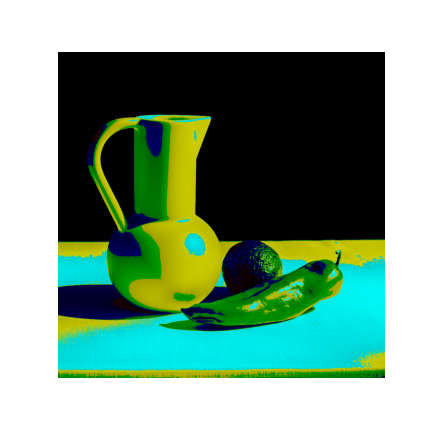
\includegraphics[scale=0.7]{images/colorized_rgb.png}
\caption{Szürkeárnyalatos kép kiszínezése RGB színtérben.}
\label{fig:colorized_rgb}
\end{figure}

Itt már szépen megjelennek az árnyékok, jól kivehetőek a színátmenetek.

\Section{HSV}

A HSV színtér szintén széles körben használt, az emberi szem számára megfelelőbb színtér. A HSV színtérben minden pixelt a következő 3 paraméter határoz meg:
\begin{itemize}
\item színárnyalat (Hue)
\item telítettség (Saturation)
\item érték (Value)
\end{itemize}

A színárnyalat (H) az alapszínt jelöli vagy fokban, vagy számokban. A színek skáláját a \ref{tab:hsv_colors}. táblázat szemlélteti.

\begin{table}[h]
\centering
\caption{HSV színtér színárnyalatainak az értéke.}
\label{tab:hsv_colors}
\medskip
\begin{tabular}{|c|c|c|}
\hline
Érték fokban & Érték számmal & Értékhez tartozó szín \\
\hline
0$^{\circ}$ vagy 360$^{\circ}$ & 0 vagy 6 & Vörös \\
\hline
60$^{\circ}$ & 1 & Sárga \\
\hline
120$^{\circ}$ & 2 & Zöld \\
\hline
180$^{\circ}$ & 3 & Cián \\
\hline
240$^{\circ}$ & 4 & Kék \\
\hline
300$^{\circ}$ & 5 & Magenta \\
\hline
\end{tabular}
\end{table}

A telítettség (S) azt írja le, hogy a szín milyen mennyiségben tartalmazza a fehér színt. A telítettséget mindig százalékos értékben adjuk meg, a 100\% jelenti a teljesen telített színt. Minél kisebb az értéke, annál halványabb a szín, mivel egyre több szürkét tartalmaz.

Az értéket (V) szokták fényerőnek (Brightness) is hívni, olyankor a színteret HSB színtérként emlegetik, de ez megegyezik a HSV színtérrel. A az érték a szín sötétségét fejezi ki százalékos arányban, ahol a 0\% a fekete, a 100\% a fehér színt jelenti. \cite{colorspaces}

A HSV színtérben található szürkeárnyalatos képek a H és S csatornákon 0 értékeket tartalmaznak, a kép csak a V értékeiből áll. Ahhoz, hogy szürkeárnyalatosból színes képet tudjunk készíteni, szükségünk van mind a H és mind az S csatorna értékeire. A \ref{fig:hsv_colorization}. ábra szemlélteti a színezés megvalósításának lehetőségeit. 

\begin{figure}[h]
\centering
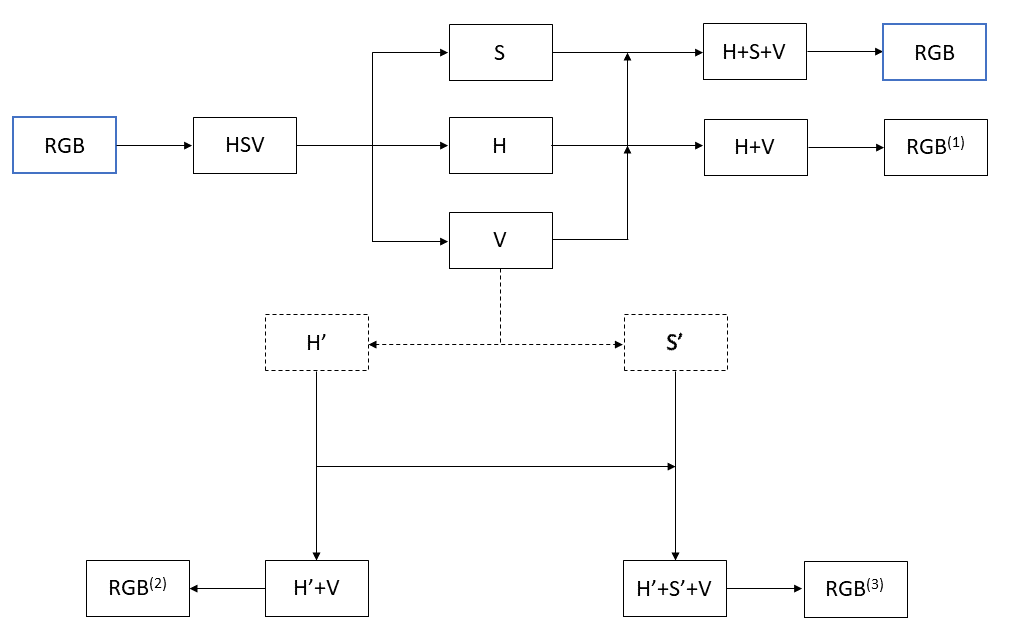
\includegraphics[scale=0.5]{images/hsv_colorization.png}
\caption{Kép színének visszabecslése HSV színtérben.}
\label{fig:hsv_colorization}
\end{figure}

Az ábra abból indul ki hogy van egy RGB színterű képünk, ezt átalakítjuk HSV színterűvé. Ha csatornáira bontjuk a képet, akkor a V  jelzi nekünk a szürkeárnyalatos képet. Amennyiben ismerjük az eredeti H és S csatornákat, akkor jól látható, hogy az eredeti képet fogjuk visszakapni. Amennyiben csak a H értékeit ismerjük, abban az esetben az $RGB^{(1)}$ kép elég hasonló, de színerősségben nagy valószínűséggel különböző lesz. Ezek azok az esetek, amikor valahonnan visszakapjuk ezeket az értékeket, például ha egyébként megvan az eredeti RGB kép és onnan meghatározzuk őket.

Amennyiben csak egy szürkeárnyalatos képünk van, abban az esetben ezeket a csatornákat valahogyan meg kell becsülnünk. Az ábrán a szaggatott vonal jelképezi a becslést, a becsült csatornákat pedig H' és S' jelöli. 

Amennyiben a H csatornát tudjuk csak megbecsülni, abban az esetben az S értékének valamilyen átlagértéket veszünk. A kapott $RGB^{(2)}$ képünk nagyban el fog térni az eredeti képtől, hiszen a színek sem biztos hogy pontosak, az árnyalatuk pedig csak egy meghatározott átlag érték, tehát ha az eredeti kép nagyon erős színeket tartalmaz vagy nagyon halvány színeket, akkor az eredmény képünk nagyon eltérő lesz tőle.

Amennyiben viszont az S értékét is vissza tudjuk becsülni, abban az esetben az $RGB^{(3)}$ valószínűleg annyira pontos nem lesz, mintha meglenne az eredeti H és S csatorna, viszont pontosabb lesz mint az $RGB^{(1)}$ illetve az $RGB^{(2)}$.

A \texttt{colors} tömb felhasználásával egyszerűen ki lehet színezni egy szürkeárnyalatos HSV színterű képet. Az RGB színeket átalakítva HSV színterű színekké megkapjuk a H, illetve az S értékét is a színnek. Ezután már csak annyi dolgunk van, hogy ezeket az értékeket átadjuk az összes pixelnek. Egy ilyen színezés megvalósításának a kódja látható a következő kódrészletben. 
\begin{python}
import colorsys

colored_image_rgb = cv2.cvtColor(resized_image, cv2.COLOR_GRAY2RGB)

hsv_image = cv2.cvtColor(colored_image_rgb, cv2.COLOR_RGB2HSV)

colored_hsv = hsv_image

for label in range(k):
    color_hsv = colorsys.rgb_to_hsv(
        colors[label][0]/255,
        colors[label][1]/255,
        colors[label][2]/255)
    for i in range(1024):
        for j in range(1024):
            if(label_map[i][j] == label):
                colored_hsv[i][j] =\
                [color_hsv[0]*180, color_hsv[1]*255, hsv_image[i][j][2]]
\end{python} 

A színek konvertálására a \texttt{colorsys} csomagot használom, abból is az \texttt{rgb\_to\_hsv} függvényt, ami bemenetként az RGB szín csatornáit várja 0 és 1 közötti értékként, ezért a szín minden értékét el kell osztani 255-tel. A meglévő szürkeárnyalatos képet átalakítom színes képpé a már korábban bemutatott módon, majd a színes képet HSV színterűvé. Ezután indítok egy for ciklust a k értékein, ami csak úgy, mint az RGB színezésnél a label értékeket fogja jelölni. Ezután a \texttt{colors} tömbből megkapott RGB színt átkonvertálom HSV színné. Minden olyan pixelt, ami a \texttt{label\_map} szerint az éppen vizsgált label értékű, kiszínezek a megadott szín szerint. A konvertálás során a HSV szín értékei 0 és 1 közötti értékek lettek, így ezeket még fel kell szorozni, hogy a megfelelő színeket kapjuk. A V értéke mindenhol marad az eredeti, szürkeárnyalatos kép V értéke.

A színezés eredménye a \ref{fig:colorized_hsv}. ábrán látható. 

\begin{figure}[h]
\centering
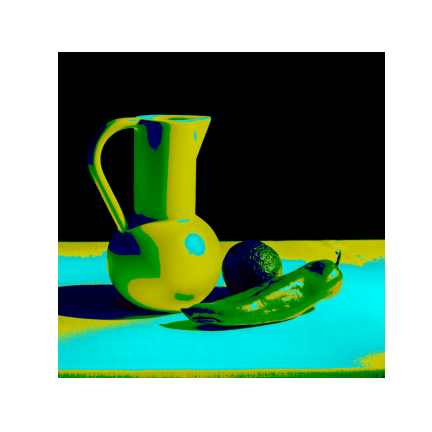
\includegraphics[scale=0.7]{images/colorized_hsv.png}
\caption{Szürkeárnyalatos kép kiszínezése HSV színtérben.}
\label{fig:colorized_hsv}
\end{figure}

A képet a kiszínezés után az egyszerű kirajzolás érdekében visszaalakítottam RGB színterűvé. Jól látható, hogy a két színtérben történő színezés ugyanazt a képet eredményezi.

\Section{Képek színének visszabecslése}

Az előző alfejezetekben bemutatott színezés során a kép színeit általam előre meghatározott színekből választottam ki. 